%\documentclass[11pt,a4paper,titlepage,twoside]{article}
\documentclass[12pt,a4paper,twoside]{article}
\usepackage{mystyle}
%\usepackage{gplot}
%\usepackage{foto_v001}
%\usepackage{mechanik_v001}

\usepackage{hyperref}
\usepackage{pdfpages}
\usepackage{pdflscape}


%\author{Felix Binder}
\title{Kernphysik}
\date{}

\newcommand{\Kern}[3]{$^{#1}_{\phantom{1}#2}\text{#3}$}
\begin{document}
\maketitle

Abschnitte dieses Dossies stammen aus dem Leitprogramms ``Radioaktivität'' der ETH Zürich.
Das vollständige Leitprogramm können Sie unter \url{http://www.educ.ethz.ch/unt/um/phy/mp/radioakt/index} finden.

\section*{Einführung}
Die Kernphysik gehört zu den neueren Entwicklungen der Physik und beschäftigt sich, wie der Name schon sagt, mit den Kernen der Atome.

\begin{aufgabe}
	Der Zeitstrahl auf der nächsten Seite zeigt auf der linken Seite technische Entwicklungen und auf der rechten Seite
	Ereignisse, die mit der Kernphysik zusammenhängen.
	Ergänzen Sie Jahreszahlen beim Zeitstrahl.
\end{aufgabe}


\newcommand{\LS}[2]{
\pgfmathsetmacro{\Datum}{0.1*(#1-1814)};
%\draw (\Datum,-0.1) -- (\Datum,0.1) node [rotate=90, left] {#2};
\draw (\Datum,-0.1) -- (\Datum,0.1) node [left] {#2};
}

\newcommand{\RS}[2]{
\pgfmathsetmacro{\Datum}{0.1*(#1-1814)};
%\draw (\Datum,0.1) -- (\Datum,-0.1) node [rotate=90, right] {#2};
%\path (\Datum,0.1) -- (\Datum,-0.1) node [right] {\phantom{#2}};
\draw (\Datum,0.1) -- (\Datum,-0.1) node [right] {#2};
}

\begin{tikzpicture}[rotate=90]
	
%Zeitleiste
\draw [->] (0,0)--(21,0);
\LS{1876}{Erstes Telefon}
\LS{1847}{Erste schweizer Eisenbahnstrecke}
\LS{1886}{Erstes Auto}
\LS{1896}{Erstes Röntgenbild}
\LS{1973}{Magnetresonanztomographie}
\LS{1945}{Zündung der ersten Atombombe}
\LS{1956}{Test einer Wasserstoffbombe}
\LS{1992}{Erstes modernes Mobilfunktelefon}
\LS{1969}{Die ersten Menschen auf dem Mond}
\LS{2007}{Erstes IPhone}
\LS{1826}{Erstes Foto der Welt}

%\RS{1895}{Entdeckung der Röntgenstrahlen}
\RS{1896}{Entdeckung der Radioaktivität}
\RS{1898}{Entdeckung des Radiums durch Marie Curie}
\RS{1905}{Spezielle Relativitätstheorie durch Albert Einstein ($E=m\cdot c^2$)}
\RS{1909}{Entdeckung des Atomkerns durch Ernest Rutherford}
\RS{1930}{Das Neutrino wird durch Wolfgang Pauli theoretisch vorausgesagt}
\RS{1932}{Entdeckung des Neutrons}
\RS{1938}{Entdeckung der erste Kernspaltung durch Otto Hahn}
\RS{1955}{Experimentelle Bestätigung des Antiprotons}
\RS{1956}{Experimentelle Bestätigung des Neutrino}
\RS{1968}{Quarks werden entdeckt}
\RS{1994}{Das Element mit Ordungszahl $Z=110$ wurde erzeugt}
\RS{2013}{Experimentelle Bestätigung des Higgs-Teilchens}
\end{tikzpicture}


\newpage



Jedes Atom besitzt einen elektrisch positiven Kern um den elektrisch negativ geladene Elektronen kreisen. Ein neutrales Atom besitzt gleich
viele positive Ladungen im Kern wie negative Ladungen in seiner Hülle.
Die Elektronen, besonders die in der äusseren Hülle bestimmen die chemischen Eigenschaften des Atoms.

Der Kern besteht aus \emph{Nukleonen}, so nennt man die Teilchen, die den Kern bilden. 
Es sind elektrisch positiv geladenen \emph{Protonen} und elektrisch neutrale \emph{Neutronen}.
Die Anzahl $Z$ der Protonen bestimmt die Art des Atoms, ein Atom mit acht Protonen ist zum Beispiel immer ein Sauerstoffatom.
Gleichnamige Ladungen stossen sich ab, deshalb braucht der Atomkern Neutronen, um die abstossende Wirkung der Protonen zu kompensieren.
Ohne diese wäre der Kern nicht stabil.
Die Anzahl der Neutronen in einem Kern wird mit $N$ angegeben.
Die Summe von Ordungszahl $Z$ und Neutronenzahl $N$ nennt man Massenzahl $A$.
Kern mit gleicher Ordungszahl und unterschiedlicher Massenzahl nennt man \emph{Isotope}.

In leichten Kernen sind etwa gleich viele Protonen wie Neutronen. 
Schwere Kerne hingegen haben mehr Neutronen als Protonen.


Atomkerne sind etwa \SI{10}{fm} im Durchmesser.
Ein fm ist ein Femtometer: $\SI{1}{fm} = \SI{1E-15}{m}$
Zum Vergleich, der Durchmesser eines Atoms ist etwa \SI{100000}{fm} gross.

\begin{aufgabe}
	Überlegen Sie sich ein Beispiel um sich die Grössenverhältnisse von Atomkern und Atomhülle besser vorzustellen.
\end{aufgabe}


%\begin{aufgabe}
%	Ordnen Sie die folgenden Entdeckungen in die Zeitleiste ein.
%Das Element mit Ordungszahl $Z=110$ wurde erzeugt,
%Entdeckung der erste Kernspaltung durch Otto Hahn,
%Entdeckung des Radiums durch Marie Curie,
%Entdeckung des Atomkerns durch Ernest Rutherford,
%Das Neutrino wird durch Wolfgang Pauli theoretisch vorausgesagt,
%Entdeckung des Neutrons,
%Entdeckung der Radioaktivität,
%Experimentelle Bestätigung des Antiprotons,
%Experimentelle Bestätigung des Neutrino,
%Spezielle Relativitätstheorie durch Albert Einstein ($E=m\cdot c^2$),
%Experimentelle Bestätigung des Higgs-Teilchens.
%Quarks werden entdeckt,
%\end{aufgabe}
%
%\begin{aufgabe}
%	Um den Atomkern zu beschreiben, wird häufig ein Tröpfchenmodel benutzt. Dabei nimmt man an, dass sich der Atomkern wie ein Wassertropfen verhält.
%	\begin{enumerate} [a)]
%		\item Zeichnen Sie drei unterschiedlich geformte Wassertropfen.
%		\item Welche Tropfenform hat die niedrigste Energie?
%	\end{enumerate}
%\end{aufgabe}

%\newpage


\section*{Bindungsenergie}

Die Energie, die notwendig ist, um die Teile eines stabilen Systems voneinander zu trennen, heisst Bindungsenergie.

Folgendes Beispiel soll dies erläutern.

Um zwei Magnetstückchen zu trennen, die infolge der magnetischen Kraft aneinander gebunden sind, 
muss man eine gewisse Arbeit leisten. Am Anfang sind die Magnetstückchen gebunden, und am Schluss
sind sie frei. Wir können die zugefügte Energie als Bindungsenergie der zwei Magnetstückchen bezeichnen.

Im Atomkern wirken zwei verschiedene Kräfte: die elektromagnetische Abstossung zwischen den Protonen
und die starke Wechselwirkung, die alle Nukleonen aneinander bindet.


Die Bindungsenergie eines Kerns ist die Arbeit, die notwendig ist, um alle Kernteile voneinander zu trennen.
Oder äquivalent: Die Bindungsenergie eines Atomkerns ist die Energie, die freigesetzt würde,
wenn man aus freien Nukleonen einen Kern bilden würde.


Die Bindungsenergie des Kernes ist viel grösser als die Arbeit, die notwendig ist, um ein Elektron von einem Atom zu trennen.

Oft benützt man auch die Bindungsenergie pro Nukleon. Sie ist definiert als das Verhältnis der Bindungsenergie des Kerns zur Anzahl seiner Nukleonen.

\begin{aufgabe}
	Die Entweichgeschwindigkeit auf der Erdoberfläche beträgt $v = \SI{11.2}{km/s}$.
	Wie gross ist die Bindungsenergie eines \SI{70}{kg} schweren Menschen?

	\kloesung{\SI{4.4}{GJ}}

	\begin{loesung}
		\begin{eqnarray*}
			\RI{E}{B}=\nicefrac{1}{2}\cdot m\cdot v^2=\SI{4390,4E6}{J}
		\end{eqnarray*}
	\end{loesung}
\end{aufgabe}


Eine grosse Bindungsenergie zu haben, bedeutet für ein System, sehr stabil zu sein. 
Man braucht nämlich viel Energie, um es auseinander zu nehmen. Ein fallendes Objekt 
sucht sich immer die tiefst mögliche Lage aus, wo die Bindungsenergie für das System
Objekt\nobreakdash-Erde am grössten ist. Auch die Nukleonen gruppieren sich möglichst
zu einer Konfiguration mit hoher Bindungsenergie, wo sie stärker gebunden sind.
Die Bindungsenergie eines Kerns hängt von der Protonenzahl Z und der Neutronenzahl N ab.
Es gibt energetisch günstige Kombinationen von (N, Z), für welche die Bindungsenergie hoch
ist, und ungünstige, für die die Bindungsenergie niedrig ist. 
%Diese Kurve liegt zuerst bei der Geraden N=Z und weicht dann davon ab in Richtung grösserer Neutronenzahl.
%Man nennt diese Kurve und ihre Umgebung auch Stabilitätstal, weil dort die stabilen Kerne liegen.

Das schwerste, noch ganz stabile Nuklid ist Bi\nobreakdash-209 (Wismut).
Darüber hinaus kennt man heute Kerne bis etwa zur Massenzahl A=270 (Z bis 110).
Wesentlich schwerere Kerne kann es nicht geben, weil die zusammenhaltende Kernkraft
nur kurze Reichweite hat, während die auseinandertreibende elektromagnetische Abstossung langreichweitig ist.



Ausnahme: Der Neutronenstern bildet eine exotische Ausnahme. 
Was diesen übergrossen {\quotedblbase}Kern{\quotedblbase} zusammenhält 
ist die Gravitationskraft. Sie ist zwar 1040mal schwächer als die Kernkraft, 
aber langreichweitig, und bei einer Masse von etwa 1057 Nukleonen (d.h. A=1057)
übertrifft sie alle anderen Kräfte (Niederer 1990, 2.5).

\subsubsection*{Wie kann man die Bindungsenergie messen?}
Wenn man die Masse aller Nukleonen eines Kerns addiert, so bekommt man einen Wert, 
der immer grösser ist als die Masse des Kerns. Diese Massendifferenz ist charakteristisch 
für jeden Kern. Sie wird Massendefekt genannt. Man kann diese Diskrepanz wie folgt verstehen: 
Nach Einstein lässt sich die Energie in Masse ausdrücken und umgekehrt. Die Gleichung lautet:

\begin{eqnarray*}
	E=m\cdot c^2
\end{eqnarray*}

Dabei ist $E$ die Energie, $m$ die Masse und $c$ die Lichtgeschwindigkeit.

Nehmen wir an, man füge einem Kern eine Energiemenge zu, die gleich seiner Bindungsenergie ist,
dann werden seine Nukleonen wieder frei. Aus der Äquivalenz von Masse und Energie entspricht
dies einer Zunahme der Masse $\Delta m = \nicefrac{\Delta E}{c^2}$.
Bilden umgekehrt zwei isolierte Nukleonen einen Kern, so wird die entsprechende Bindungsenergie freigesetzt.
Dies entspricht nach Einstein einem Massenschwund  $\Delta m = \nicefrac{\Delta E}{c^2}$.

\begin{figure}[h]
	\centering
	\includegraphics[width=0.90\textwidth]{./Binding_energy_curve_-_common_isotopes_DE.pdf}
	\caption{Bindungsenergie pro Nukleon}
	\label{fig:Bindungsenergie_pro_Nukleon}
\end{figure}


In Abbildung \ref{fig:Bindungsenergie_pro_Nukleon} ist die Bindungsenergie pro Nukleon für stabilere Kerne gezeigt. 
(1eV (Elektronenvolt) ist ein Mass für die Energie in der Atom- und Kernphysik:
$\SI{1}{eV} = \SI{1.6E-19}{J}$. Also: $\SI{1}{MeV} = \SI{1.6E-13}{J}$.
Diese Energie ist am grössten für Kerne mit Massenzahl um 60 (Fe: Eisen).
Für schwerere Kerne nimmt die Bindungsenergie pro Nukleon ab. Der Grund ist,
dass die zusammenhaltende Kraft unter den Nukleonen (die starke Wechselwirkung) eine sehr kurze Reichweite hat,
während die abstossende Kraft unter den Protonen (elektromagnetische Kraft) langreichweitig ist.
Deshalb spürt ein Proton die Abstossung aller anderen Protonen, auch der weit entferntesten,
aber nur die Anziehung der unmittelbar nahen Nukleonen.

 


Wir berechnen die Bindungsenergie von $\text{Fe}^{56}$ (Eisen). 
Die Nukleonenzahl A ist 56. Aus Abbildung \ref{fig:Bindungsenergie_pro_Nukleon} lesen wir ab,
dass die Bindungsenergie pro Nukleon für $Fe^{56}$ ca. \SI{8.6}{MeV} beträgt. 
Somit hat $Fe^{56}$ eine totale Bindungsenergie $\RI{E}{B} = 56\cdot\SI{8.6}{MeV} = \SI{481.6}{MeV}$.




\begin{aufgabe}
	\begin{enumerate} [a)]
		\item Beschreiben Sie in einem Sätzen was die Bindungsenergie ist.
		\item Welche Wechselwirkung (Kraft) hält die Atomkerne zusammen? Welche Wechselwirkung (Kraft) wirkt gegen das Zusammenhalten?
		%\item Wie erklärt der Artikel die relativ schwache Bindung der leichten Kerne?
		\item Welcher Kern hat die höchste Bindungsenergie pro Nukleon im Atomkern? Wie hoch ist diese Energie in Joule?
		\item Warum kann man die Bindungsenergie kurzlebiger Kerne aus deren Zerfallsprodukten bestimmen?
		\item Wo in der Grafik stehen die Kerne, die sich fusionieren lassen? Wo die, die bei der Spaltung Energie freigeben? Können Sie das erklären?
	\end{enumerate}
\end{aufgabe}

\begin{aufgabe}
	In der Abbildung \ref{fig:Bindungsenergie_pro_Nukleon} ist $^3_2\text{He}$ und $^3_1\text{H}$ aufgeführt. 
	Welches der beiden sollte stabiler sein? Stimmt das?
\end{aufgabe}

\begin{aufgabe}
	Berechnen Sie mit Hilfe der Abbildung \ref{fig:Bindungsenergie_pro_Nukleon} die Bindungsenergie des \Kern{16}{8}{O} Kerns.
\end{aufgabe}


\begin{aufgabe}
	Nehmen Sie an ein Kern der Massenzahl $A=240$ wird in zwei Kerne der mit der Massenzahl $A=120$ gespalten. 
	Bestimmen Sie aus der Abbildung \ref{fig:Bindungsenergie_pro_Nukleon} die dabei	freiwerdende Energie.
\end{aufgabe}

\begin{aufgabe}
	In der Sonne werden Wasserstoffkerne zu Heliumkernen fusioniert.
	Wie viel Energie wird dabei frei. Benutzen Sie die \ref{fig:Bindungsenergie_pro_Nukleon} zum Lösen der Aufgabe.
\end{aufgabe}

\newpage

\section*{Radioaktivität}

Die Aufgaben auf dieser Seite sind als Ergänzung des Kapitels 2: Radioaktivität, des Leitprogramms ``Radioaktivität'' der ETH Zürich zu verstehen.
Das vollständige Leitprogramm können Sie unter http://www.educ.ethz.ch/unt/um/phy/mp/radioakt/index finden.


\subsubsection*{Übersicht}
Im Jahre 1896 entdeckte Becquerel bis dahin unbekannte Strahlen. Diese neuen ``radioaktiven'' Strahlen 
wurden intensiv erforscht und die gewonnenen Erkenntnisse in der Kerntechnologie vielfältig umgesetzt.
Die anfänglich euphorische Zustimmung musste einer allgemeinen Skepsis weichen.
Heute ist der Begriff ``Radioaktivität'' in aller Munde. Die Diskussion ist im Gange.
Die Meinungen sind geteilt und oft festgefahren. Steigen Sie ein, diskutieren Sie mit!
Dieses Kapitel bietet Ihnen den physikalischen Hintergrund dazu.

%Nachdem Sie das Kapitel durchgearbeitet haben,
%werden Sie die wichtigsten Strahlenarten beschreiben können.
%Hier lernen Sie die wichtigsten Grössen und Hilfsmittel zur Charakterisierung der radioaktiven Strahlung kennen.
%
%Einfache praktische Anwendungen runden das Kapitel ab.

%\subsubsection*{Vorgehen}
%Studieren Sie zuerst die Lernziele. Nachdem Sie sich die wesentlichen Ziele gemerkt haben, steigen Sie ins Kapitel ein.
%
%Den grössten Teil des Kapitels bearbeiten Sie alleine. Bei einem Experiment und einer Lernaufgabe arbeiten Sie mit Partnern zusammen. 
%
%Auch in diesem Kapitel werden Sie zum Literaturstudium aufgefordert. Gehen Sie, wenn Sie so weit sind, zur Handbibliothek. Der Lehrer hat Ihnen dort alle Bücher bereitgestellt.
%
%Im Text befinden sich einige Aufgaben. Hier können Sie Ihr Verständnis und Ihre Fähigkeiten testen. Die Lösungen zu diesen Aufgaben finden Sie am Ende des Kapitels.
%
%Die Lernkontrolle beim Kapitelende vermittelt Ihnen die letzte Sicherheit. Die Lösungen dazu stehen auf der folgenden Seite. Wenn Sie 3 dieser 4 Kontrollfragen richtig beantwortet haben, melden Sie sich beim Lehrer zum Kapiteltest.
%
%Viel Spass!
%
%
%\bigskip
%
%\clearpage
%\bigskip
%



%Lernziele
%1.\ \ Sie können die drei wichtigsten Zerfallsarten nennen und den Aufbau der dabei ausgesandten Teilchen beschreiben.
%
%2.\ \ Sie können in wenigen Sätzen die Begriffe {\quotedblbase}Aktivität{\quotedblbase} und {\quotedblbase}Halbwertszeit{\quotedblbase} mit eigenen Worten beschreiben. Denn dies sind zwei besonders bedeutende Grössen. Sie wissen, wie sich die Aktivität einer Probe zeitlich verändert und können diese Kenntnisse bei einfachen Berechnungsaufgaben anwenden.
%
%3.\ \ Sie haben den Umgang mit der Nuklidkarte intensiv geübt. Aufbau und Anwendungsbeispiele sind Ihnen geläufig. Beim Lösen verschiedener Aufgaben stellen Sie Ihre Kenntnisse unter Beweis.
%
\subsection*{Einleitung}


``Radioaktivität'' ist in aller Munde. Doch was versteht man darunter?

Das Duden Fremdwörterbuch schreibt dazu:
\begin{cbox}
Radioaktivität:\\
Eigenschaft der Atomkerne gewisser Isotope, sich ohne äussere Einflüsse umzuwandeln und dabei bestimmte Strahlen auszusenden.
\end{cbox}

Nun ein bisschen mehr dazu.

\subsubsection*{Die Entdeckung der Radioaktivität}

Becquerel entdeckte 1896, dass Uransalze auch bei vollkommener Dunkelheit eine Photoplatte durch seine lichtdichte
Verpackung hindurch zu schwärzen vermochten. Becquerel schloss, dass die Schwärzung nur durch eine vom Uransalz 
stammende Strahlung verursacht werden konnte. Er nannte diese Strahlung dann auch ``Uranstrahlung''.

Kurz darauf fand das Ehepaar Curie, dass weitere Minerale zum Teil noch wesentlich stärker strahlten.
Alle diese Materialien brauchten nicht zuerst zum Strahlen angeregt zu werden.
Sie strahlten spontan und selbständig. Pierre und Marie Curie prägten für dieses
``aktive'' Strahlen den Begriff ``Radioaktivität''.

%Sind Sie speziell an Becquerels Biographie interessiert? Einen kurzen und interessanten Artikel finden Sie in: Schenk, E.: {\quotedblbase}Mein Name ist Becquerel{\quotedblbase} auf den Seiten 30ff.

Heute kennt man rund 1500 verschiedene Nuklide. 
Lediglich 249 davon sind stabil (nicht radioaktiv). 
Der Rest sind instabile Radionuklide (radioaktive Nuklide). 
Diese erstrecken sich über alle Elemente. 
Das heisst es gibt kein Element, das nicht mindestens ein radioaktives Isotop besässe.

\subsubsection*{Woher stammt die ionisierende Strahlung?}


Um diese Frage beantworten zu können, wurden viele Versuche durchgeführt. Dazu wurden u.a.:

\begin{itemize}
	\item die verschiedensten Substanzen (chemische Verbindungen) untersucht,
	\item die Proben extremen Temperaturen ausgesetzt,
	\item die Proben extremen Drücken ausgesetzt
\end{itemize}

und vieles mehr.

All diese Versuche beeinflussen die Elektronenhülle der untersuchten Atome. 
Doch die Strahlung wurde durch diese Veränderungen nicht beeinflusst. 
Einzig die Anzahl der vorhandenen radioaktiven Kerne war für die Intensität (Stärke) der Strahlung ausschlaggebend.

Schlussfolgerung: Die Strahlung wird nicht aus der Atomhülle emittiert. Die Strahlung muss aus dem Kern stammen.

\subsubsection*{Natürliche Strahlung, künstliche Strahlung}

Von den ca. 1500 heute bekannten Nukliden kommen rund 500 in der Natur seit Milliarden Jahren vor. 
249 davon sind stabil, der Rest ist radioaktiv. Die Strahlung, die beim Zerfall dieser Radionuklide
ausgesandt wird, nennen wir natürliche ionisierende Strahlung.

Die restlichen rund 1000 Nuklide gibt es jedoch erst wieder,
seit dem sich der Mensch mit Kernforschung und Kerntechnik auseinandersetzt. 
Dies sind rund 100 Jahre. Diese Nuklide sind künstlich entstanden. Sie alle sind radioaktiv. Die Strahlung dieser Gruppe Radionuklide wird künstliche ionisierende Strahlung genannt.

Warum heisst es oben ``erst wieder seit rund 100 Jahren''? Was war denn vorher?

Die künstlichen Nuklide sind eigentlich gar nicht neu. Sie gab es schon früher einmal. 
In der Zwischenzeit waren sie jedoch auf der Erde ausgestorben. Diese künstlich erzeugten Nuklide
sind nämlich alle radioaktiv. Doch ihre Lebensdauer ist kurz. Das heisst, sie haben die vielen Milliarden Jahre,
die seit ihrer Entstehung vergangen waren, nicht überlebt.
Darum fand man sie auch nicht mehr in der Natur. Jetzt gibt es sie wieder.

Doch nicht nur der Mensch erzeugt solche Radionuklide. Auch heute werden noch derartige Nuklide im Universum erzeugt.
Die Theorie sagt nämlich, dass alle im Universum vorkommenden Elemente, die eine höhere Atommasse als Eisen aufweisen,
in Supernovaen (explodierende Sterne grosser Masse) entstanden sein müssen.

\begin{aufgabe}
Aus welchem Teil des Atoms stammen die radioaktiven Strahlen?
\end{aufgabe}


\subsection*{Strahlenarten}


Es gibt verschiedene Arten radioaktiver Strahlen. 
Diese lassen sich in mehrere Gruppen einteilen. 
In diesem Abschnitt werden Sie die drei wichtigsten Strahlenarten kennen lernen.

Rutherford entdeckte schon 1898, dass es mindestens zwei Arten radioaktiver Strahlen geben muss (Segrè 1981, 61).
Er nannte diese $\alpha$- und $\beta$-Strahlen. Später wurden als weitere Sorte die $\gamma$-Strahlen entdeckt. 

Man führte verschiedene Experimente mit diesen Strahlen durch. 
Unter anderem untersuchte man auch deren elektrisches und magnetisches Verhalten %(Abbildung 2.1).
Hier die Ergebnisse:
\begin{itemize}
	\item $\alpha$-Strahlen sind doppelt geladene Heliumkerne.
	\item $\beta$-Strahlen lassen sich leicht durch Magnetfelder ablenken. Sie verhalten sich wie Elektronen.
	\item $\gamma$-Strahlen passieren die magnetischen und elektrischen Felder unbeeinflusst. Sie verhalten sich wie Lichtstrahlen.
\end{itemize}



%\ \   [Warning: Image ignored] % Unhandled or unsupported graphics:
%\includegraphics[width=8.961cm,height=15.381cm]{radio-img/radio-img021.wmf}
 

%Abbildung 2.1: Ablenkung der \textgreek{a}\nobreakdash-, \textgreek{b} \nobreakdash- und \textgreek{g} \nobreakdash-Strahlen im Magnetfeld.


\subsubsection*{Der Alpha-Zerfall}

1904 wurde bekannt, dass bei Radiumverbindungen, die $\alpha$-Strahlen aussenden, 
Helium auftritt. Dieses Helium konnte nur beim Zerfall des Radiums entstanden sein. 
Alle weiteren Versuche führten zur folgenden Feststellung:

Beim $\alpha$-Zerfall werden Teilchen ausgesandt.
Alle diese Teilchen bestehen aus 2 Protonen und aus 2 Neutronen. 
Diese Teilchen sind also Heliumkerne.

Die ausgesandten Teilchen werden $\alpha$-Teilchen genannt.


%Abbildung 2.2: Schematische Darstellung des \textgreek{a} \nobreakdash-Zerfalls

Nach einem $\alpha$-Zerfall fehlen dem ursprünglichen Nuklid 2 Protonen und 2 Neutronen. 
Das ursprüngliche Element hat sich also durch den Zerfall in ein neues gewandelt.

\begin{aufgabe}
Radon-222 (\Kern{222}{86}{Rn}) sendet beim Zerfall ein $\alpha$-Teilchen aus. In welches Element wandelt sich das Radon durch diesen Zerfall?
Lösen Sie die Aufgabe mit Hilfe des Periodensystems.
\end{aufgabe}


\subsubsection*{Der Beta-Zerfall}


Beim $\beta$-Zerfall werden ebenfalls Teilchen ausgesandt. 
Diese Teilchen verhalten sich wie Elektronen. Zum Beispiel werden sie, dank ihrer kleinen Masse,
leicht in Magnetfeldern abgelenkt. Man nennt diese Teilchen $\beta$-Teilchen.

Es gibt 2 Sorten von $\beta$-Teilchen.

Bei den einen stimmen Masse, Ladung und Verhalten genau mit denen der Elektronen überein.
Hier werden also Elektronen ausgesandt. Eine derartige Strahlung heisst $\beta^-$-Strahlung. 
(Sprich: ``Beta-Minus-Strahlung''. Minus weil das emittierte Elektron negativ geladen ist.)

Die zweite Sorte der ausgesandten Teilchen unterscheidet sich von den Elektronen lediglich durch ihre Ladung. 
Elektronen sind negativ geladen. Diese Teilchen jedoch sind positiv geladen. 
Sie werden Positronen genannt. Eine derartige Strahlung heisst denn auch $\beta^+$-Strahlung 
(Sprich: ``Beta-Plus-Strahlung'').

Woher stammen diese Elektronen und Positronen? Gibt es im Kern freie Elektronen oder Positronen?

Nein, im Kern gibt es weder freie Elektronen noch freie Positronen. 
Überlegungen der Quantenphysik, auf die wir hier nicht näher eingehen, sagen, dass Elektronen und Positronen im Kern nicht frei existieren können.

Experimente haben aber gezeigt, dass sich Neutronen in Protonen und Protonen in Neutronen umwandeln können. 
Bei diesen Umwandlungen entstehen dann die gesuchten Elektronen beziehungsweise Positronen.

Betrachten wir eine solche Umwandlung. In diesem Beispiel soll ein Proton in ein Neutron umgewandelt werden. 
Wir wissen, das Proton ist positiv geladen, das Neutron ist ungeladen. Bei der Umwandlung muss also noch ein Teilchen entstehen,
das die positive Ladung aufnehmen kann. Sonst wäre die Gesamtladung nach der Umwandlung nicht gleich der Gesamtladung vor der Umwandlung.
(Denn auch hier gilt das Gesetz der Ladungserhaltung. Dieses besagt, dass bei jedem Umwandlungsprozess die Summe der Ladungen erhalten bleiben muss.)
Das Positron erfüllt diese Aufgabe. Es hat die gleiche Masse wie ein Elektron, ist jedoch positiv geladen.

Da es keine freien Positronen im Kern geben kann, werden diese nach der Entstehung sofort aus dem Kern emittiert.

In Kurzform lautet diese Reaktion:\\
\begin{eqnarray*}
	p^+ \to n + e^+ + \nu
\end{eqnarray*}


Ursprünglich glaubte man, der $\beta$-Zerfall verletze das Gesetz der Energieerhaltung. Heute weiss man mehr:

\begin{enumerate}
\item Das beim $\beta^-$-Zerfall erzeugte Proton und das freigesetzte Elektron haben eine
	kleinere Totalenergie als das ursprüngliche Neutron. Beim $\beta$-Zerfall entsteht aber noch ein drittes Teilchen.
	Dieses wird Anti-Neutrino ($\nu$) genannt. Es wird ebenfalls aus dem Kern emittiert und trägt den Rest der Energie,
	die beim Zerfall entsteht, mit sich. Das Anti-Neutrino ist ungeladen. Weil die Totalenergie der Teilchen nach dem
	Zerfall (Proton, Elektron, Anti-Neutrino) kleiner ist als vor dem Zerfall (Neutron) ist ein freies Neutron instabil (radioaktiv).

\item Das beim $\beta^+$-Zerfall erzeugte Neutron und das freigesetzte Positron haben eine kleinere Totalenergie
	als das ursprüngliche Proton. Beim $\beta^+$-Zerfall entsteht ebenfalls ein drittes Teilchen. Dieses wird Neutrino
	($\nu$) genannt. Es wird aus dem Kern emittiert und trägt den Rest der Energie, die beim Zerfall frei wird, mit sich.
	Das Neutrino ist ungeladen. Weil die Totalenergie der Teilchen nach dem Zerfall (Neutron, Positron, Neutrino) grösser
	ist als vor dem Zerfall (Proton) ist ein freies Proton stabil. Die für den $\beta^+$-Zerfall nötige Energie stammt
	aus der höheren Bindungsenergie des übrigbleibenden Atomkerns.
\end{enumerate}

\begin{aufgabe}
Stelle die Reaktionsgleichung für die Umwandlung eines Neutrons in ein Proton auf. ( Achtung: Das Antineutrino nicht vergessen.)
\end{aufgabe}



Wie beim $\alpha$-Zerfall wird auch beim $\beta$-Zerfall der Kern verändert.
Das heisst die Substanzen (Elemente) vor und nach dem Zerfall sind nicht mehr die selben.

\begin{itemize}
	\item Beim $\beta^-$-Zerfall geht ein Neutron des Kerns in ein Proton über.
		Die Ordnungszahl des Kerns erhöht sich um 1. Dadurch entsteht ein anderes chemisches Element.

	\item Beim $\beta^+$-Zerfall geht ein Proton des Kerns in ein Neutron über.
		Die Ordnungszahl senkt sich um 1. Auch hier ändert das chemische Element.
\end{itemize}


%  [Warning: Image ignored] % Unhandled or unsupported graphics:
%\includegraphics[width=10.513cm,height=6.279cm]{radio-img/radio-img024.wmf}
 

%Abbildung 2.3: Schematische Darstellung des b\nobreakdash-Zerfalls

\begin{aufgabe}
C-14 ist ein $\beta^-$-Strahler. Das heisst, C-14 emittiert beim Zerfall ein Elektron.
In welches Element verwandelt sich der Kohlenstoff durch den Zerfall?
Lösen Sie die Aufgabe mit Hilfe des Periodensystems. 
\end{aufgabe}



\subsubsection*{Die Gamma-Strahlung}
Nach einem $\alpha$- oder $\beta$-Zerfall ist der Kern oft in einem angeregten Zustand.
Das heisst, im Kern befindet sich noch Energie, die abgebaut werden sollte.
Dieser Energieabbau erfolgt durch Aussenden elektromagnetischer Strahlung.

Diese Strahlung hat die gleiche Natur wie sichtbares Licht. 
Auch Licht ist eine elektromagnetische Strahlung. 
Doch die $\gamma$-Strahlung ist viel kurzwelliger und darum viel energiereicher als das Licht.

Der angeregte Kern gibt jedoch seine Energie nicht kontinuierlich ab. $\gamma$-Strahlen 
werden in einzelnen Portionen (Quanten) ausgesandt.
Die Physiker sagen, es wird ein Photon oder $\gamma$-Quant ausgesandt.

%  [Warning: Image ignored] % Unhandled or unsupported graphics:
%\includegraphics[width=10.513cm,height=6.35cm]{radio-img/radio-img025.wmf}
 

%Abbildung 2.4: Schematische Darstellung des \textgreek{g}\nobreakdash-Zerfalls

Obwohl kein eigentlicher Kernzerfall stattfindet, sprechen die Physiker auch hier von einem Zerfall,
dem $\gamma$-Zerfall. In dieser Sprechweise könnten Sie etwa sagen: 
``Der angeregte (energiereiche) Zustand des Kerns zerfällt in einen energieärmeren Zustand und in ein $\gamma$-Quant,
das ausgesandt wird''.

Beim $\gamma$-Zerfall werden die Nukleonen des Kerns weder umgewandelt noch ausgesandt.
Das bedeutet, dass vor und nach dem Energieabbau das gleiche Element vorhanden ist. Der Kern strahlt einzig Energie ab.


\subsection*{Aktivität}


Sie wissen, dass Radionuklide spontan zerfallen und dabei Teilchen aussenden. 
Wenn Sie zum Beispiel eine Salatprobe vor sich haben, 
möchten Sie aber auch sagen können, wie oft in dieser Probe ein Zerfall stattfindet.
Sie brauchen also ein Mass, das beschreibt, wie intensiv Ihre Probe strahlt. Zu diesem Zweck definieren wir die Aktivität:

%Definition 2.1

\begin{eqnarray*}
	\text{Aktivität}=\frac{\text{Anzahl Kernzerfälle}}{\text{Zeiteinheit}}
\end{eqnarray*}


Die Einheit der Aktivität ist 1 Becquerel = 1 Zerfall/Sekunde: [A] = 1 Bq.

%Im folgenden wollen wir die Zerfallsgesetze im Detail herleiten. Sie können jetzt Ihr mathematisches Wissen gut gebrauchen.

%Wenn Sie ein paar einfache Regeln der Differentialrechnung gelernt haben, 
%dann machen Sie mit den folgenden Abschnitten weiter, es lohnt sich! 
%Falls Sie keine Grundkenntnisse der Differentialrechnung haben, gehen Sie direkt zur Zusammenfassung.
%
%Der radioaktive Zerfall hat rein statistischen Charakter. Wir können nur für eine sehr, 
%sehr grosse Zahl von radioaktiven Nukliden, aber nicht für ein einzelnes Nuklid, voraussagen, 
%wann der Zerfall eintritt. Wir führen deshalb die Zerfallswahrscheinlichkeit $l$ dafür ein,
%dass ein bestimmter Kern pro Zeiteinheit zerfällt. $l$ hat die Einheit 1/s.
%
%In einer Menge $N$ identischer radioaktiver Kerne ist also die gesamte Zahl der Zerfälle pro Zeiteinheit $N\cdot l$.
%
%%\ \   [Warning: Image ignored] % Unhandled or unsupported graphics:
%%\includegraphics[width=5.151cm,height=1.094cm]{radio-img/radio-img027.wmf}
%% \ \ (2.1)
%
%\begin{eqnarray*}
%	A = N\cdot\lambda=-\frac{dN}{dt}
%\end{eqnarray*}
%
%Die Anzahl der radioaktiven Kerne nimmt mit der Zeit ab, 
%da ja immer einige Kerne zerfallen. Wir nehmen dabei an, dass ein Kern nach dem Zerfall stabil sei.
%
%%\ \   [Warning: Image ignored] % Unhandled or unsupported graphics:
%%\includegraphics[width=9.807cm,height=1.199cm]{radio-img/radio-img028.wmf}
% 
%\begin{eqnarray*}
%	A=-\frac{dN}{dt}=-\lim_{\Delta t\to 0} \frac{\RI{N}{nachher} -\RI{N}{vorher}}{\Delta t}, \RI{N}{nachher} < \RI{N}{vorher}
%\end{eqnarray*}
%
%Merken Sie, warum das Minuszeichen da sein muss?
%
%Die Gleichung 
%\begin{eqnarray*}
%	N\cdot\lambda=-\frac{dN}{dt}
%\end{eqnarray*}
%nennt man eine Differentialgleichung 1. Ordnung. 
%Gesucht ist die Anzahl der Kerne $N(t)$, welche diese Gleichung erfüllt. Anfangsbedingung: $N(t=0)=N_0$.
%
%\begin{flushleft}
%\tablefirsthead{}
%\tablehead{}
%\tabletail{}
%\tablelasttail{}
%\begin{supertabular}{m{3.8009999cm}m{1.301cm}m{9.801001cm}}
%Lösungsweg: &
%~
% &
%  [Warning: Image ignored] % Unhandled or unsupported graphics:
%%\includegraphics[width=2.822cm,height=0.706cm]{radio-img/radio-img030.wmf}
% \\
%~
% &
%~
% &
%  [Warning: Image ignored] % Unhandled or unsupported graphics:
%%\includegraphics[width=2.399cm,height=1.094cm]{radio-img/radio-img031.wmf}
% \\
%~
% &
%~
% &
%Beide Seiten integrieren:
%
%  [Warning: Image ignored] % Unhandled or unsupported graphics:
%%\includegraphics[width=2.787cm,height=1.094cm]{radio-img/radio-img032.wmf}
% \\
%~
% &
%~
% &
%  [Warning: Image ignored] % Unhandled or unsupported graphics:
%%\includegraphics[width=2.681cm,height=0.564cm]{radio-img/radio-img033.wmf}
% \\
%~
% &
%~
% &
%Anfangsbedingung: N(t=0)=N0\\
%~
% &
%~
% &
%  [Warning: Image ignored] % Unhandled or unsupported graphics:
%%\includegraphics[width=5.503cm,height=0.6cm]{radio-img/radio-img034.wmf}
% \\
%~
% &
%~
% &
%  [Warning: Image ignored] % Unhandled or unsupported graphics:
%%\includegraphics[width=3.246cm,height=0.6cm]{radio-img/radio-img035.wmf}
% \\
%~
% &
%~
% &
%  [Warning: Image ignored] % Unhandled or unsupported graphics:
%%\includegraphics[width=3.316cm,height=0.6cm]{radio-img/radio-img036.wmf}
% \\
%~
% &
%~
% &
%  [Warning: Image ignored] % Unhandled or unsupported graphics:
%%\includegraphics[width=2.081cm,height=1.199cm]{radio-img/radio-img037.wmf}
% \\
%~
% &
%${\Rightarrow}$ &
%  [Warning: Image ignored] % Unhandled or unsupported graphics:
%%\includegraphics[width=2.505cm,height=0.706cm]{radio-img/radio-img038.wmf}
% \ \ Zerfallsgesetz\ \ (2.2)\\
%\end{supertabular}
%\end{flushleft}
%

%$N(t) = \text{Zahl der zur Zeit} t \text{noch vorhandenen Kerne}$.
%
%Da die Aktivität $A = N\cdot \lambda$ ist, gilt:
%
%\begin{eqnarray*}
%	A = N\cdot \lambda = N_0\cdot\exp{-\lambda\cdot t} = A_0\cdot\exp{-\lambda\cdot t}
%\end{eqnarray*}
%\begin{eqnarray*}
%	A(t)=A_0\cdot\exp{-\lambda\cdot t}
%\end{eqnarray*}
%
%Die Aktivität nimmt zeitlich mit dem gleichen Gesetz ab wie die Anzahl der radioaktiven Kerne.

\subsubsection*{Zusammenfassung}
Der radioaktive Zerfall hat rein statistischen Charakter. 
Man kann also von einem Kern nicht sagen, wann er zerfällt, sondern nur, wie gross die Wahrscheinlichkeit ist, 
dass er in einer gewissen Zeitspanne zerfällt. Damit gleichbedeutend ist die Aussage, 
wie viele Zerfälle aus einer riesigen Anzahl von Nukliden stattfinden.

Wie viele radioaktive Kerne in einer gewissen Zeit zerfallen, hängt von zwei Grössen ab:

\begin{itemize}
	\item Zum einen ist dies die Anzahl vorhandener Kerne. Denn, je mehr Kerne vorhanden sind, desto mehr können auch zerfallen.
	\item Zum anderen ist es die Zerfallswahrscheinlichkeit. Sie ist ein Mass dafür, wie ``gerne'' ein Kern zerfällt.
\end{itemize}


Diese Art von Abhängigkeit wird durch eine Exponentialfunktion beschrieben:

\begin{eqnarray*}
	N(t)=N_0\cdot\exp{(-\lambda\cdot t)}
\end{eqnarray*}

Dabei ist $N(t)$ die Anzahl radioaktiver Kerne zur Zeit t,
$N_0$ ist die Ursprüngliche Anzahl radioaktiver Kerne und
$\lambda$ ist die Zerfallswahrscheinlichkeit. Die Einheit der Zerfallswahrscheinlichkeit ist [$\lambda$] = $s^{-1}$.

Die Aktivität ist proportional zur Anzahl radioaktiver Kerne. Die Proportionalitätskonstante ist die Zerfallswahrscheinlichkeit.

\begin{eqnarray*}
	A(t) = \lambda\cdot N(t)=A_0\cdot \exp{(-\lambda\cdot t)}
\end{eqnarray*}
%\ \   [Warning: Image ignored] % Unhandled or unsupported graphics:
%\includegraphics[width=4.586cm,height=0.635cm]{radio-img/radio-img043.wmf}
wobei $A_0= \lambda\cdot N_0$ ist.

\begin{aufgabe}
	
	Eine Probe mit 1 mg reinem Radium-226 (\Kern{226}{88}{Ra}) hat etwa \num{2.7E18} Kerne. 
	Die Zerfallswahrscheinlichkeit beträgt \SI{13.8E-12}{s^{-1}}.
%	(Dies entspricht einer Halbwertszeit von 1600 Jahren. Mehr darüber lernen Sie im Abschnitt 2.4).

	\begin{enumerate}[a)]
		\item Wie gross ist die Aktivität dieser Probe?
		\item Wie viele Kerne zerfallen in 15 Minuten?
		\item Wie gross ist die Aktivität noch nach diesen 15 Minuten?
	\end{enumerate}

\end{aufgabe}


%Experiment 2.1
%
%Der Lehrer hat Ihnen ein Experiment vorbereitet. 
%
%In diesem Experiment sollten Sie den zeitlichen Verlauf der Aktivität einer Pa\nobreakdash-234\nobreakdash- oder einer anderen geeigneten Probe aufnehmen, das Ergebnis graphisch darstellen und interpretieren.
%
%Arbeiten Sie zu zweit. Suchen Sie sich einen Partner, der im Leitprogramm gerade etwa am selben Ort steht wie Sie. Planen und führen Sie das Experiment gemeinsam durch.
%
%\subsubsection*{Was geschieht in diesem Experiment?}
%Die Probe zerfällt und sendet \textgreek{b}\nobreakdash-Teilchen aus. Ein bestimmter Anteil aller ausgesandten Strahlen löst im Detektor einen elektrischen Impuls aus. Diese Impulse werden registriert. Ihre Anzahl wird fortlaufend aufaddiert und angezeigt.
%
%\subsubsection*{Was ist Ihre Aufgabe?}
%Bestimmen Sie den zeitlichen Verlauf der Aktivität der bereitgelegten Probe. Stellen Sie die Ergebnisse Ihrer Messung graphisch dar, und diskutieren Sie das Resultat. Ihre Messung sollte den Aktivitätsverlauf über einen Zeitraum von rund 5 Minuten wiedergeben.
%
%\subsubsection*{Wie gehen Sie vor?}
%Bedienung der Geräte:
%
%Lassen Sie sich von Ihrem Betreuer oder von Ihrer Betreuerin die wesentlichen Elemente der Messapparatur und deren Bedienung erläutern. Beachten Sie auch die Geräteanleitung.
%
%Planung des Experiments:
%
%Planen Sie Ihr gemeinsames Vorgehen. Achtung, während der Messung könnte es hektisch werden. Arbeiten Sie deshalb zu zweit. Besprechen Sie mit Ihrem Partner Ihr Vorgehen. Wer macht wann genau was? Erstellen Sie vor Messbeginn die nötigen Unterlagen.
%
%Haben Sie schon eine gemeinsame Strategie zur Durchführung der Messung erarbeitet? Falls nicht, finden Sie im nächsten Abschnitt zwei kurze Vorschläge.
%
%Durchführung des Experimentes:
%
%Wenn alles bereit ist, starten Sie die Messung. Protokollieren Sie alle Zwischenergebnisse. Unterlassen Sie in dieser Phase jegliche Auswerteschritte.
%
%Auswertung des Experimentes:
%
%Beginnen Sie die Auswertung erst nach Beendigung der Messung. Erstellen Sie die Graphik. Tragen Sie dazu die registrierten Impulse in Abhängigkeit der Zeit auf. Beschreiben Sie in höchstens zwei kurzen Sätzen den beobachteten zeitlichen Verlauf der Aktivität.
%
%Nun beantworten Sie folgende Frage: Durch welche mathematische Funktion könnte das Abklingen der Aktivität angenähert werden?
%
%\subsubsection*{Zwei Vorschläge zum praktischen Vorgehen.}
%Die einen setzen den Zähler zuerst auf 0. Nach Messbeginn lassen sie ihn dann frei hochzählen. In periodischen Abständen Dt lesen Sie den Zählerstand ab und notieren sich die Werte. Die Aktivität erhalten sie, indem sie den aktuellen Wert minus den vorangegangenen Wert nehmen und die Differenz durch die Periodendauer teilen.
%
%Die anderen führen periodische Intervallmessungen durch. Sie setzen den Zählerstand auf 0. Dann starten sie die Messung. Diese wird nach beispielsweise 5 Sekunden gestoppt. Der Wert wird abgelesen, der Zähler wird zurückgesetzt. In periodischen Abständen folgen die nächsten Messequenzen. Die Aktivität erhält man, indem der Wert einer Intervallmessung durch die Dauer seines Messintervalls geteilt wird.
%
%\subsubsection*{Ergebnis}
%Mit zunehmender Zeit wird die Aktivität immer schwächer. Dabei scheint die Aktivität exponentiell abzufallen. Die Kurve lässt sich recht gut durch eine Exponentialkurve annähern (Abbildung 2.5).
%
%  [Warning: Image ignored] % Unhandled or unsupported graphics:
%%\includegraphics[width=15.91cm,height=10.585cm]{radio-img/radio-img044.wmf}
% 
%
%Abbildung 2.5: Aktivitätsverlauf einer Pa\nobreakdash-234 Probe
%
%Diese Exponentialkurve stellt aber nur einen Mittelwert dar. Denn beim radioaktiven Zerfall handelt es sich um Zufallsereignisse. Das heisst, dass während einer Messperiode einmal mehr, einmal weniger Kerne zerfallen als im Mittel. Bestimmt man die Aktivität in ganz kurzen Zeiteinheiten (Feinbestimmung), kann man diese Abweichungen sichtbar machen (vergleiche Abbildung 2.6).
%
%  [Warning: Image ignored] % Unhandled or unsupported graphics:
%%\includegraphics[width=15.951cm,height=10.585cm]{radio-img/radio-img045.wmf}
% 
%
%Abbildung 2.6: Feinbestimmung des Aktivitätsverlaufs einer Pa\nobreakdash-234 Probe
%
\begin{aufgabe}
	C-11 ist ein $\beta^{+}$-Strahler. In welches Element wandelt sich das Kohlenstoff durch den Zerfall?
\end{aufgabe}

\begin{aufgabe}
	Das Bild zeigt einen Ausschnitt aus einer Nuklidkarte. 
	Zeigen Sie durch Pfeile, wohin das Mutternuklid durch $\alpha$-, $\beta^{-}$- und $\beta^{+}$-Zerfall zerfällt?

	\begin{center}
		
	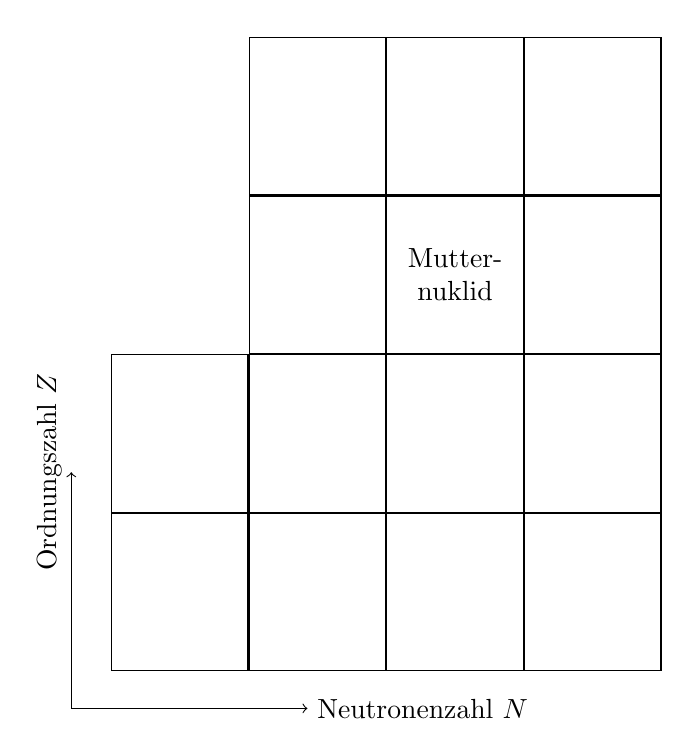
\begin{tikzpicture}
\matrix (N)[every node/.style={draw, text width=1.5cm, align=flush center, minimum height=2cm}]
{
& \node (){}; & \node {}; & \node {}; \\
& \node (){}; & \node {Mutter-nuklid}; & \node {}; \\
\node {}; &\node (){}; & \node {}; & \node {}; \\
\node (UL) []{}; &\node (){}; & \node {}; & \node {}; \\};
\draw [->](-4,-4.5) --++(0:3cm) node [right] {Neutronenzahl $N$};
\draw [->](-4,-4.5) --++(90:3cm) node [rotate=90, above] {Ordnungszahl $Z$};
	\end{tikzpicture}
	\end{center}

\end{aufgabe}

\begin{aufgabe}
	Die Isotope, die in der Isotopenkarte links von den stabilen Isotope stehen, sind oft $\beta^{+}$-Strahler.
	Die Isotope rechts der stabilen Isotope sind oft $\beta^{-}$-Strahler. Wie können Sie sich das erklären?
\end{aufgabe}

\begin{aufgabe}
	Beim Zerfall eines Radium-222 Kerns in einen Radon-118 Kern 
	wird ein Heliumkern frei ($\alpha$-Strahler).
	\begin{enumerate}[a)]
		\item Welche kinetische Energie hat der Heliumkern?
		\item Welcher Geschwindigkeit entspricht das?
	\end{enumerate}
	Tipp: Es gilt Energieerhaltung.

	\Kern{222}{88}{Ra}: \SI{222.0153618}{u} 
	mit einer Bindungsenergie von \SI{1708677.123}{keV}.

	\Kern{218}{86}{Rn}: \SI{218.0055863}{u}
	mit einer Bindungsenergie von \SI{1687062.361}{keV}.

	$^4_2\text{He}$: \SI{4.0026032}{u}
	mit einer Bindungsenergie von \SI{28295.673}{keV}

	\kloesung{a) \SI{6.681}{MeV}, b) \SI{17.9E6}{m/s}}

\end{aufgabe}

\newpage
\begin{aufgabe}\label{ZerfallendeSchüler}
	Stellen Sie sich vor alle Schüler in der Klasse sind radioaktive Kerne, die mit der Zeit zerfallen können.
	Ob ein Schüler zerfällt oder nicht wird beim Würfeln entschieden. Würfelt ein Schüler eine 6, so zerfällt er und setzt sich hin.
    In jeder Runde würfeln alle noch aktiven Kerne.

Bestimmen Sie die Anzahl der stehenden Schüler für die ersten fünf Würfelrunden.
\end{aufgabe}

\subsection*{Halbwertszeit \RI{T}{1/2}}

Die Zerfallskonstante ist eine unanschauliche Grösse. Deshalb führen wir die Halbwertszeit \RI{T}{1/2} ein.

Die Halbwertszeit besagt, nach welcher Zeit sich die Zahl der Nuklide und damit die Aktivität halbiert haben wird.

Nach Ablauf einer zweiten Halbwertszeit hat sich die Zahl der Nuklide erneut halbiert. 
Sie ist nun die Hälfte der Hälfte, also ein Viertel. Nach dem Verstreichen einer weiteren Halbwertszeit
beträgt die Nuklidzahl ein Achtel, dann ein Sechzehntel usw. Mathematisch zusammengefasst lässt sich schreiben:

\begin{eqnarray*}
	N(t) = N_0\cdot 2^{\nicefrac{t}{\RI{T}{1/2}}}
\end{eqnarray*}

beziehungsweise für die Aktivität

\begin{eqnarray*}
	A(t) = A_0\cdot 2^{\nicefrac{t}{\RI{T}{1/2}}}
\end{eqnarray*}

%
%Nochmals zu Ihrem Experiment (Experiment 2.1) zurück. Bestimmen Sie die Halbwertszeit des dort verwendeten radioaktiven Präparats. Beschreiben Sie Ihr Vorgehen zur Bestimmung der Halbwertszeit in wenigen Worten. Schreiben Sie höchstens 3 kurze Sätze.
%
\begin{aufgabe}
	
Fiktive Annahme:
Vor 10 Milliarden Jahren hätten \SI{1E13}{kg} (10 Milliarden Tonnen) Pu-244 existiert. 
In der Zwischenzeit wäre jedoch dieses Plutonium ständig zerfallen. 
Pu-244 ist eines der langlebigsten künstlichen Elemente. Seine Halbwertszeit beträgt \num{8.3E7} Jahre.

Welche Masse wäre von diesen ursprünglichen \SI{1E13}{kg} Pu-244 heute noch vorhanden?
\end{aufgabe}

%\subsubsection*{Lernaufgabe}
\subsubsection*{Beziehung zwischen der Halbwertszeit und der Zerfallskonstanten}
Zwischen der Halbwertszeit und der Zerfallskonstanten gilt eine einfache Beziehung. 
Diese herauszufinden ist Ihre Aufgabe. Dazu eine kleine Hilfe: 
Nach Verstreichen einer Halbwertszeit wird die ursprüngliche Anzahl Radionuklide auf die Hälfte geschrumpft sein. Es gilt:

\begin{eqnarray*}
	t=\RI{T}{1/2}\qquad\text{und}\qquad N(\RI{T}{1/2}) =\frac{N_0}{2}\text{.}
\end{eqnarray*}



Durch einsetzen erhalten Sie

\begin{eqnarray*}
	\frac{N_0}{2}=N_0\cdot \exp{(-\lambda\cdot\RI{T}{1/2})}\text{.}
\end{eqnarray*}

\begin{aufgabe}
Ermitteln Sie nun daraus den Zusammenhang zwischen der Halbwertszeit und der Zerfallskonstanten. 
Lösen Sie dazu diese Gleichung nach $\lambda$ auf.
\end{aufgabe}



\begin{aufgabe}
	Wie gross ist Halbwertszeit in Aufgabe \ref{ZerfallendeSchüler}.
\end{aufgabe}


\begin{aufgabe}
	In Physiklabor haben wir also radioaktive Proben Ra-226.
	Bestimmen Sie mit der Nuklidkarte die vollständige Zerfallsreihe dieses Elements.
\end{aufgabe}


%Den Lösungsvorschlag zu dieser Aufgabe finden Sie auf der nächsten Seite.
%
%\subsubsection*{Lösungsvorschlag}
%Zuerst eliminieren Sie N0. Sie erhalten
%
%\ \   [Warning: Image ignored] % Unhandled or unsupported graphics:
%%\includegraphics[width=2.328cm,height=1.164cm]{radio-img/radio-img051.wmf}
% 
%
%Nach beidseitigem Logarithmieren folgt
%
%\ \   [Warning: Image ignored] % Unhandled or unsupported graphics:
%%\includegraphics[width=3.21cm,height=0.706cm]{radio-img/radio-img052.wmf}
% 
%
%Durch Umformen erhalten Sie für die Beziehung zwischen der Zerfallskonstanten und der Halbwertszeit
%
%\ \   [Warning: Image ignored] % Unhandled or unsupported graphics:
%%\includegraphics[width=2.223cm,height=1.235cm]{radio-img/radio-img053.wmf}
% \ \ ( 2.7 )
%
%\subsection[2.5 Nuklidkarte]{2.5 Nuklidkarte}
%
%\bigskip
%
%Die Nuklidkarte ist ein wichtiges Hilfsmittel der Kernphysik.
%
%\subsubsection*{Literaturstudium}
%Zum Aufbau der Nuklidkarte lesen Sie in Dorn, Bader: {\quotedblbase}Physik in einem Band{\quotedblbase} auf Seite 533, {\quotedblbase}§196 Die Nuklidkarte{\quotedblbase}.
%
%Studieren Sie unbedingt die Graphik auf den Seiten 578 und 579.
%
%Aufgabe 2.8
%
%Die Felder der Nuklidkarte sind farbig. Jede Farbe repräsentiert einen bestimmten Zerfallstyp. Durch welche Farben werden a\nobreakdash-, b\nobreakdash-\nobreakdash- und b+\nobreakdash-Zerfälle wiedergegeben?
%
%
%\bigskip
%
%\subsubsection*{Lernaufgabe}
%\subsubsection*{Anwendung der Nuklidkarte}
%Gewisse Radionuklide senden bei der Umwandlung Teilchen aus. Dabei wandeln sich die Atome von einem Element zum anderen. Wir sagen: Aus der Mutter entsteht durch den Zerfall die Tochter. Der Mutter-Tochter-Übergang kann auf der Nuklidkarte nachvollzogen werden. Jede der betrachteten Zerfallsarten, bei denen Nukleonen ausgesandt oder umgewandelt werden (\textgreek{a}, \textgreek{b}\nobreakdash-, \textgreek{b}+), entspricht einem typischen Verschiebungsmuster auf der Karte. Dieses Verschiebungsmuster sollten Sie herausfinden und sich einprägen.
%
%Vorbereitung:
%
%Wissen Sie noch, welche Kernreaktionen beim \textgreek{a}\nobreakdash-, \textgreek{b}\nobreakdash-\nobreakdash-, \textgreek{b}+\nobreakdash-Zerfall stattfinden? Wenn nicht schauen Sie in Abschnitt 2.2 nach.
%
%\subsubsection*{1. Teil der Aufgabe}
%Erstellen Sie eine Tabelle und tragen Sie für jede der 3 Zerfallsarten (\textgreek{a}, \textgreek{b}\nobreakdash-, \textgreek{b}+) die Änderung
%
%{\textbullet}\ \ der Gesamtzahl aller Nukleonen (Nukleonenzahl A)
%
%{\textbullet}\ \ der Anzahl Protonen (Ordnungszahl Z)
%
%{\textbullet}\ \ der Neutronenzahl (Neutronenzahl N)
%
%auf.
%
%\begin{flushleft}
%\tablefirsthead{}
%\tablehead{}
%\tabletail{}
%\tablelasttail{}
%\begin{supertabular}{m{2.3009999cm}m{4.801cm}m{4.801cm}}
%Beispiel: &
%\textgreek{a}{}-Zerfall &
%~
%\\
%~
% &
%A geht über in A\nobreakdash-4: &
%A ${\rightarrow}$ A\nobreakdash-4\\
%~
% &
%N geht über in ... &
%N ${\rightarrow}$ ...\\
%~
% &
%Z geht über in ... &
%Z ${\rightarrow}$ ...\\
%\end{supertabular}
%\end{flushleft}
%Das Vervollständigen ist Ihre Aufgabe.
%
%\subsubsection*{2. Teil der Aufgabe}
%Diese Zerfälle führen auf der Nuklidkarte zu einem typischen Verschiebungsmuster. Erstellen Sie dazu eine {\quotedblbase}Kurzanleitung{\quotedblbase}. Notieren Sie sich zu jeder Zerfallsart, wie Sie auf der Nuklidkarte vom Mutternuklid zum Tochternuklid gelangen.
%
%Beispiel:
%
%Wir betrachten den Übergang N ${\rightarrow}$ N+1.
%
%Kurzanleitung: Ausgehend vom Ausgangsnuklid gelangen wir zum Zielnuklid, indem wir auf der Karte ein Feld nach rechts rücken.
%
%\subsubsection*{1. Lösungsvorschläge}
%\subsubsection*{Teil 1:}
%\begin{flushleft}
%\tablefirsthead{}
%\tablehead{}
%\tabletail{}
%\tablelasttail{}
%\begin{supertabular}{m{3.8500001cm}m{3.8500001cm}m{3.8500001cm}m{3.8500001cm}}
%${\alpha}$\nobreakdash-Zerfall: &
%A${\rightarrow}$A\nobreakdash-4 &
%N${\rightarrow}$N\nobreakdash-2 &
%Z${\rightarrow}$Z\nobreakdash-2\\
%${\beta}$\nobreakdash-\nobreakdash-Zerfall: &
%A${\rightarrow}$A &
%N${\rightarrow}$N\nobreakdash-1 &
%Z${\rightarrow}$Z+1\\
%~
% &
%(unverändert) &
%~
% &
%~
%\\
%${\beta}$+\nobreakdash-Zerfall: &
%A${\rightarrow}$A &
%N${\rightarrow}$N+1 &
%Z${\rightarrow}$Z\nobreakdash-1\\
%~
% &
%(unverändert) &
%~
% &
%~
%\\
%\end{supertabular}
%\end{flushleft}
%\subsubsection*{Teil 2:}
%Von der Muttersubstanz gelangen Sie zur Tochtersubstanz, indem Sie auf der Nuklidkarte
%
%\begin{flushleft}
%\tablefirsthead{}
%\tablehead{}
%\tabletail{}
%\tablelasttail{}
%\begin{supertabular}{m{3.3009999cm}m{4.801cm}m{6.801cm}}
%${\alpha}$\nobreakdash-Zerfall: &
%2 Felder nach links und &
%2 Felder nach unten rücken\\
%${\beta}$\nobreakdash-\nobreakdash-Zerfall: &
%1 Feld nach links und &
%1 Feld nach oben rücken\\
%${\beta}$+\nobreakdash-Zerfall: &
%1 Feld nach rechts und &
%1 Feld nach unten rücken\\
%\end{supertabular}
%\end{flushleft}
%
%\bigskip
%
%Aufgabe 2.9
%
%Welches sind die Tochterprodukte von C\nobreakdash-13, Pb\nobreakdash-202, Ra\nobreakdash-220 und N\nobreakdash-18?
%
%
%\bigskip
%
%\subsection[2.6 Zerfallsreihen]{2.6 Zerfallsreihen}
%
%\bigskip
%
%Die meisten Mutter-Tochter-Übergänge enden bei einer wiederum radioaktiven Tochter. Diese zerfällt erneut. Und vielleicht zerfällt das aus der Tochter entstandene Produkt nochmals. Dies geht weiter, bis ein stabiles Nuklid erreicht wird. So entsteht eine Zerfallsreihe.
%
%Beispiel einer solchen Zerfallsreihe: 
%
%Beispiel 2.1
%
%Die Zerfallsreihe von Radon\nobreakdash-213 lautet:
%
%Rn\nobreakdash-213 ${\rightarrow}$ Po\nobreakdash-209 ${\rightarrow}$ Pb\nobreakdash-205 ${\rightarrow}$ Tl\nobreakdash-205
%
%Aufgabe 2.10
%
%Erstellen Sie mit Hilfe der Nuklidkarte die Zerfallsreihe zu Am\nobreakdash-243. Schreiben Sie die Reihe entsprechend dem obigen Beispiel.
%
%Hier die ersten Gedankenschritte:
%
%Sie starten beim Feld Am\nobreakdash-243. Das Feld ist gelb. Am\nobreakdash-243 ist also ein a\nobreakdash- Strahler. Zur Tochter gelangen Sie, indem Sie 2 Felder nach links und zwei Felder nach unten rücken. Das ist ... und ist ein ...\nobreakdash-Strahler. Zur Tochter dieses Nuklids gelangen Sie ...
%
%
%\bigskip
%
%Es gibt 3 natürliche Zerfallsreihen. Diese werden auch {\quotedblbase}Natürliche radioaktive Familien{\quotedblbase} genannt. Jede dieser Reihen beginnt bei einem sehr langlebigen Radionuklid. Die Ausgangsnuklide dieser drei Reihen sind: Th\nobreakdash-232, U\nobreakdash-235 und U\nobreakdash-238.
%
%\subsubsection*{Lernaufgabe}
%\subsubsection*{Natürliche Zerfallsreihen}
%Bestimmen Sie das chemische Element bei dem alle drei natürlichen Zerfallsreihen enden.
%
%Vorgehen: Setzen Sie sich mit 2 Kollegen zusammen. Jeder von Ihnen erstellt eine Zerfallsreihe. Dabei wählt jeder ein anderes Ausgangsnuklid. Diskutieren Sie Ihre Resultate.
%
%\subsubsection*{Lösung}
%Alle drei natürlichen Zerfallsreihen enden beim Element Blei. Genauer:
%
%{\textbullet}\ \ Die Thorium\nobreakdash-232 Reihe endet bei Blei\nobreakdash-208.
%
%{\textbullet}\ \ Die Uran\nobreakdash-235 Reihe endet bei Blei\nobreakdash-207.
%
%{\textbullet}\ \ Die Uran\nobreakdash-238 Reihe endet bei Blei\nobreakdash-206.
%
%
%
%
%
%
%
%
%
%
%
%
%
%
%
%Periodensystem und Nuklidkarte
%\begin{landscape}
%\includepdf[pages={1}]{./periodic-table-of-chemical-elements.pdf}
%\end{landscape}

%\includepdf[pages={1-2}]{./Nuklidkarte.pdf}


\end{document}
